 \newpage
 \section{Resultados}
 
 \subsection{HPO}
 Esta enfermedad, Trombosis Arterial, está definida como HPO:0004420, manteniendo relación con otras 26 enfermedades y con 34 genes asociados.
 
 \subsection{STRING}
 Con la base de datos biológica STRING, hemos obtenido los genes asociados y sus interacciones.
\begin{figure}[h]
	\centering
	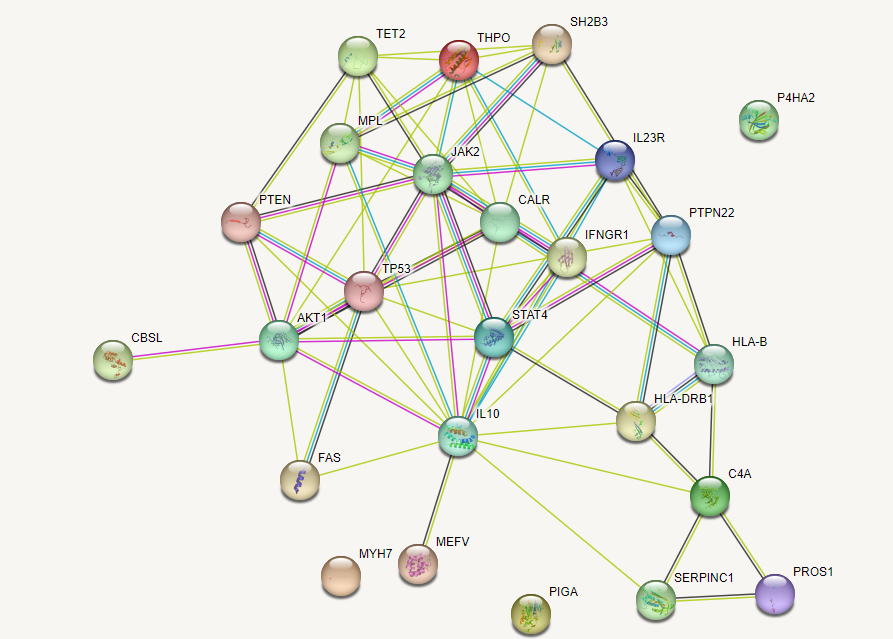
\includegraphics[width=0.70\textwidth]{figures/genes_asociados.png}
	\caption{Genes asociados a la trombosis.}
	\label{fig: Figura 3}
\end{figure}


\subsection{Comunidades}
Se han obtenido un total de 18 comunidades, siendo dos de ellas indepentientes.

En la figura 4 podemos ver una matriz con los miembros de cada comunidad. En el lateral derecho podemos ver el número de comunidades a la que pertenece cada gen mientras que en el borde inferior podemos ver el número de genes que conforma cada comunidad. 

\begin{figure}[h]
	\centering
	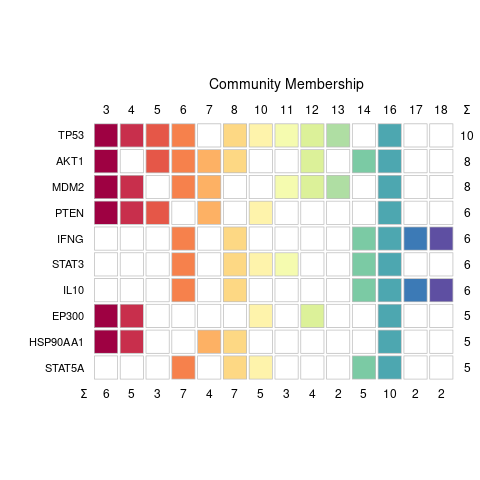
\includegraphics[width=0.70\textwidth]{figures/03_GenesMasCOnectadosOtrasComunidades.png}
	\caption{Matriz de genes por comunidad}
	\label{fig: Figura 4}
\end{figure}

En la figura 5 podemos ver los genes con mayor centralidad

\begin{figure}[h]
	\centering
	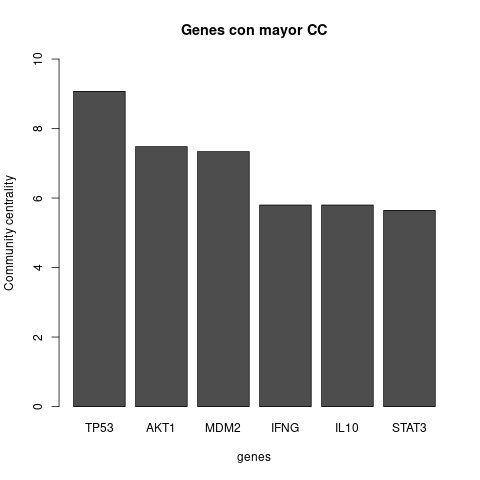
\includegraphics[width=0.70\textwidth]{figures/04_GenesMayorCentralidad.png}
	\caption{Genes con mayor centralidad}
	\label{fig: Figura 5}
\end{figure}

Por último, en la figura 6 podemos ver una red de los genes divididos por comunidades y las dos comunidades independientes.

\begin{figure}[h]
	\centering
	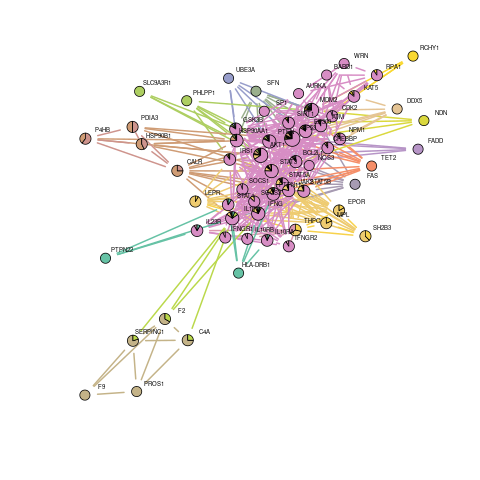
\includegraphics[width=0.70\textwidth]{figures/01_NetworkComunidades.png}
	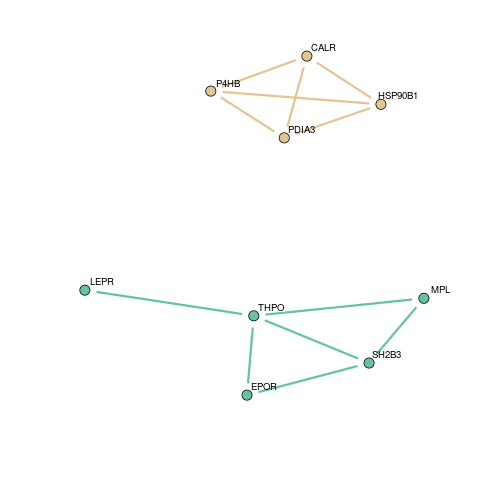
\includegraphics[width=0.70\textwidth]{figures/05_Comunidades_Independientes.png}
	\caption{Genes por comunidades y comunidades independientes}
	\label{fig: Figura 6}
\end{figure}

\subsection{Enriquecimiento de las comunidades}
Se ha realizado el enriquecimiento a todas las comunidades, los ficheros .csv se pueden visualizar en el GitHub en la carpeta 'results'.

